\documentclass[xcolor=table]{beamer}

\usepackage[french]{babel}
\usepackage[latin1]{inputenc}
\usepackage[normalem]{ulem}
\usepackage[T1]{fontenc}
\usepackage{fancyhdr}   %% Pour la gestion des num�ros de page
\usepackage{graphicx}
\usepackage{amsmath}
\usepackage{mathrsfs}
\usepackage{amsfonts}
\usepackage{palatino}        %% Palatino fonts
\usepackage{mathptm}        %% PostScript Type 1 math fonts
\usepackage{dsfont} %% Pour mathds
\usepackage{color}
%%\usepackage{pstricks}
\usepackage{xmpmulti}
\usepackage{hyperref}
\usepackage{multimedia}
\usepackage{multirow}
%\usepackage[table]{xcolor}
\usepackage{fourier-orns}
\usepackage{subfigure}
\usepackage{tikz}

\DeclareMathAlphabet{\mathpzc}{OT1}{pzc}{m}{it}

\definecolor{vert}{rgb}{0.07,0.7,0.00}
\definecolor{gris}{gray}{0.70}
\definecolor{gris2}{gray}{0.95}
\definecolor{bleu}{rgb}{0.19,0.19,0.68}

%table setting
\newcommand\T{\rule{0pt}{2.6ex}}
\newcommand\B{\rule[-1.2ex]{0pt}{0pt}}
\renewcommand{\thesubfigure}{\thefigure.\arabic{subfigure}}

\usetheme{allee_marine} %voir fichier beaerthemeallee_marine.sty   ==> \usetheme{allee_marine}


%%%%%%%%%%%%%%%%%%%%%%%%%% Pr�sentation du document %%%%%%%%%%%%%%%%%%%%%%%%%%
\title[Master 1 Project]{Indexing big colored image bank : Texture 3.0}
\author[Etienne CAILLAUD, Thomas LE BRIS, Ibrahima GUEYE, Gaetan ADIER]{\textbf{Etienne CAILLAUD, Thomas LE BRIS, Ibrahima GUEYE, Gaetan ADIER}}
\institute [XLIM-SIC UMR CNRS 7252]{\textbf{XLIM-SIC Laboratory UMR CNRS 7252, Poitiers, France}}
\date{}

%%%%%%%%%%%%%%%%%%%%%%% Num�ro de pages en bas � gauche %%%%%%%%%%%%%%%%%%%%%%
\addtobeamertemplate{footline}{\color{blue}\hfill\insertframenumber/\inserttotalframenumber}

\pgfdeclareimage[height=96mm,width=128mm]{nombidon}{mood_eye_light}
\setbeamertemplate{background}{\pgfuseimage{nombidon}}

\pgfdeclareimage[height=96mm,width=128mm]{nombidon2}{mood_eye_light}
\setbeamertemplate{background}{\pgfuseimage{nombidon2}}

%%----------------------------------------------------------------------------
%% A chaque d�but de sous-section : g�n�re une table des mati�res
%%----------------------------------------------------------------------------
\AtBeginSection[]
{
   \setbeamertemplate{background}{\pgfuseimage{nombidon}}
   \begin{frame}<beamer>
    \frametitle{Outline}
    \tableofcontents[currentsection, hideallsubsections] %% affiche la section courante et les autres en gris�, masque les sous-sections
   \end{frame}
  \setbeamertemplate{background}{\pgfuseimage{nombidon2}}
}

\AtBeginSubsection[]
{
  \setbeamertemplate{background}{\pgfuseimage{nombidon}}
  \begin{frame}<beamer>
    \tableofcontents[sectionstyle=show/shaded,subsectionstyle=show/shaded/hide, subsubsectionstyle =hide]
  \end{frame}
   \setbeamertemplate{background}{\pgfuseimage{nombidon2}}
}

\AtBeginSubsubsection[]
{
  \setbeamertemplate{background}{\pgfuseimage{nombidon}}
  \begin{frame}<beamer>
    \tableofcontents[sectionstyle=show/shaded,subsectionstyle=show/shaded/hide,subsubsectionstyle =show/shaded/hide]
  \end{frame}
   \setbeamertemplate{background}{\pgfuseimage{nombidon2}}
}


%%%%%%%%%%%%%%%%%%%%%%%%%%%%%%%%%%%%%%%%%%%%%%%%%%%%%%%%%%%%%%%%%%%%%%%%%%%%%%
%%%%%%%%%%%%%%%%%%%%%%%%%%%%                       %%%%%%%%%%%%%%%%%%%%%%%%%%%
%%%%%%%%%%%%%%%%%%%%%%%%%%     D�BUT DU DOCUMENT     %%%%%%%%%%%%%%%%%%%%%%%%%
%%%%%%%%%%%%%%%%%%%%%%%%%%%%                       %%%%%%%%%%%%%%%%%%%%%%%%%%%
%%%%%%%%%%%%%%%%%%%%%%%%%%%%%%%%%%%%%%%%%%%%%%%%%%%%%%%%%%%%%%%%%%%%%%%%%%%%%%
\begin{document}
\graphicspath{{images/}}
\setbeamercolor{block title example}{bg = gray}

\begin{frame}
    \vspace{-1.5cm}
    \begin{tikzpicture}[remember picture,overlay]
        \node[xshift=0cm, above=8.6cm] at (current page.south west)
        {
\includegraphics[width=40cm,height=0.9cm]{cache_titre.png}};
        \node[xshift=2cm, above=2.8cm] at (current page.south west)
        {
\includegraphics[height=1.5cm]{Xlim.png}};
        \node[xshift=11cm, above=3cm] at (current page.south west)
        {
\includegraphics[height=1cm]{logo_une.jpg}};
        \node[xshift=6.5cm, above=0.7cm] at (current page.south west)
        {
\includegraphics[height=1.6cm]{Lifeclef.png}};
    \end{tikzpicture}
    \titlepage
\end{frame}

%%%%%%%%%%%%%%%%%%%%%%%%%%%%%%%%%%%%%%%%%%%%%%%%%%%%%%%%%%%%%%%%%%%%%%%%%%%%%%%%%%%%%%%%%%%%%%%%%%%%%
%%%%%%%%%%%                        D�but de la pr�sentation                       			 %%%%%%%%
%%%%%%%%%%%%%%%%%%%%%%%%%%%%%%%%%%%%%%%%%%%%%%%%%%%%%%%%%%%%%%%%%%%%%%%%%%%%%%%%%%%%%%%%%%%%%%%%%%%%%
\section{Introduction}
%%-----------------------------------------------------------------------------------------
\begin{frame} \frametitle{Context and environment}

\end{frame}


\section{Team presentation}

\begin{frame} \frametitle{Deadlines}
XLIM-SIC Laboratory of University of Poitiers
\begin{itemize}
\item Noel Richard ( Researcher in Color images): Supervisor
\item David Helbert ( Researcher in Signal-Image-Communications): Supervisor
\item Thierry Urruty ( Researcher in Color images): Customer
\end{itemize}

\end{frame}
%%-----------------------------------------------------------------------------------------

\section{User requirement}
\begin{frame} \frametitle{Software}
\begin{itemize}
 \item Design  software programs:\\
   indexation of  images database,calculate descriptor according to  nature images
\item Adapt the last up to date designed color and texture attributes to the current image classification
\item Compare our results (using CLEF challenge metrics)
\item Provide an abstract of the comparisons and a technical report
\end{itemize}






%%-----------------------------------------------------------------------------------------
\end{frame}
%%-----------------------------------------------------------------------------------------

\section{Work achievement}
%%-----------------------------------------------------------------------------------------
\begin{frame} \frametitle{SIFT(Scale-Invariant Feature Transform)}

Key-points detection (x,y,$\sigma$)
\begin{itemize}

\item Scale-space extrema detection\\
Find the best locations which characterize well the image

 \item  Key-point location\\
 Improve the position of the keypoints detected

\item Orientation assignment\\
 Assign orientations to the key-points

\item key-point descriptor \\
Describe the key-point with with a vector of 128 dimension
\end{itemize}
\end{frame}

\begin{frame} \frametitle{SIFT(Scale-Invariant Feature Transform)}
\begin{figure}[htbp]
    \begin{minipage}[c]{.45\linewidth}
      \begin{center}
	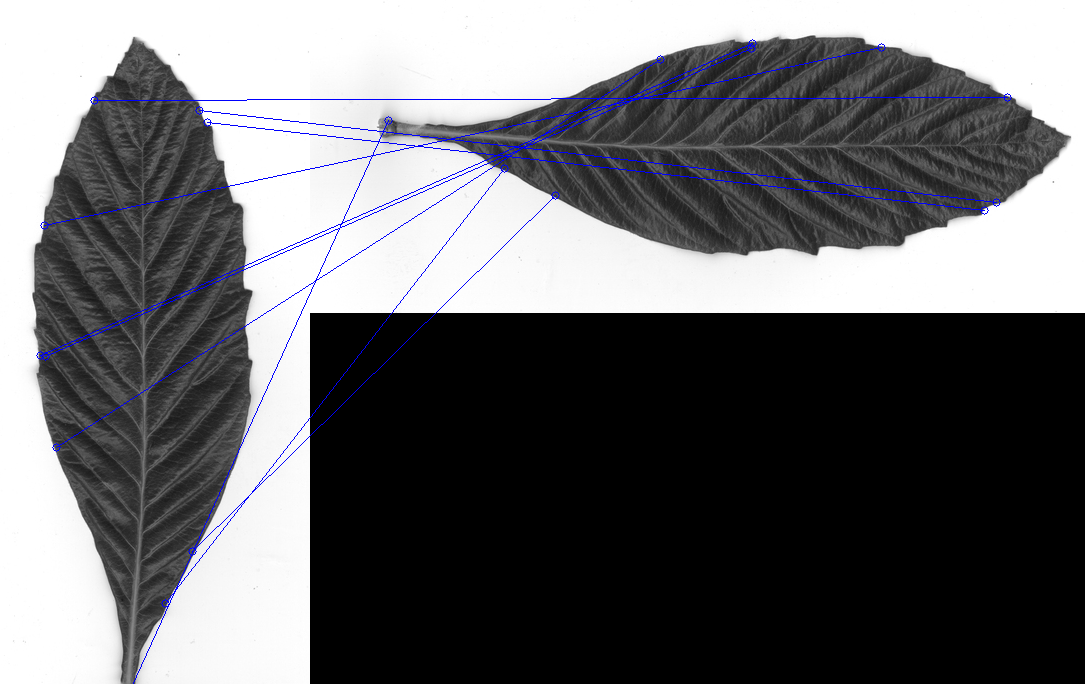
\includegraphics[scale=0.20]{Capture1.png}
	\caption{SIFT test1}
	\label{figure:Illustration}
      \end{center}
    \end{minipage}
    \hfill
    \begin{minipage}[c]{.45\linewidth}
      \begin{center}
	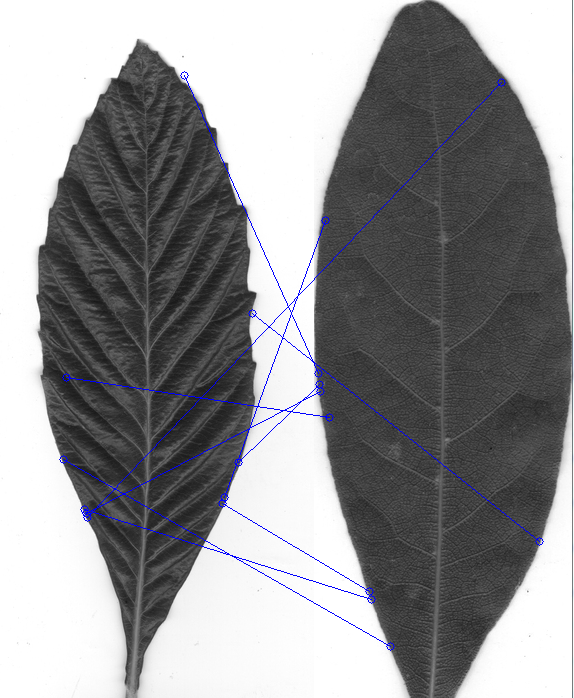
\includegraphics[scale=0.20]{Capture.png}
	\caption{SIFT test2}
	\label{figure:Illustration}
      \end{center}
    \end{minipage}
  \end{figure}
\end{frame}
%%-----------------------------------------------------------------------------------------

\begin{frame} \frametitle{C$_2$O}

\end{frame}
%%-----------------------------------------------------------------------------------------

\begin{frame} \frametitle{Classification (Bag of words)}
Reducing the number of points.

\begin{figure}[htbp]
    \begin{minipage}[c]{.55\linewidth}
      \begin{center}
        \begin{itemize}
            \item K-means
            \begin{itemize}
                \item Attribute the vectors to centroid vectors.
            \end{itemize}
        \end{itemize}
      \end{center}
    \end{minipage}
    \hfill
    \begin{minipage}[c]{.40\linewidth}
      \begin{center}
    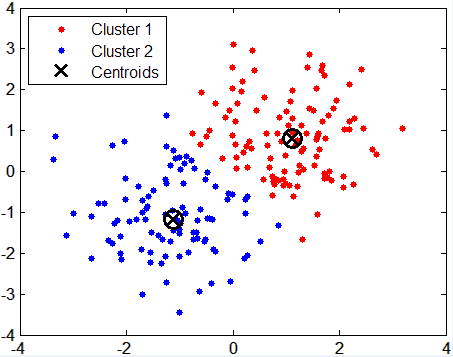
\includegraphics[scale=0.20]{kmeans.png}
    \caption{K-means}
    \label{fig:kmeans}
      \end{center}
    \end{minipage}
\end{figure}

\begin{figure}[htbp]
    \begin{minipage}[c]{.40\linewidth}
      \begin{center}
    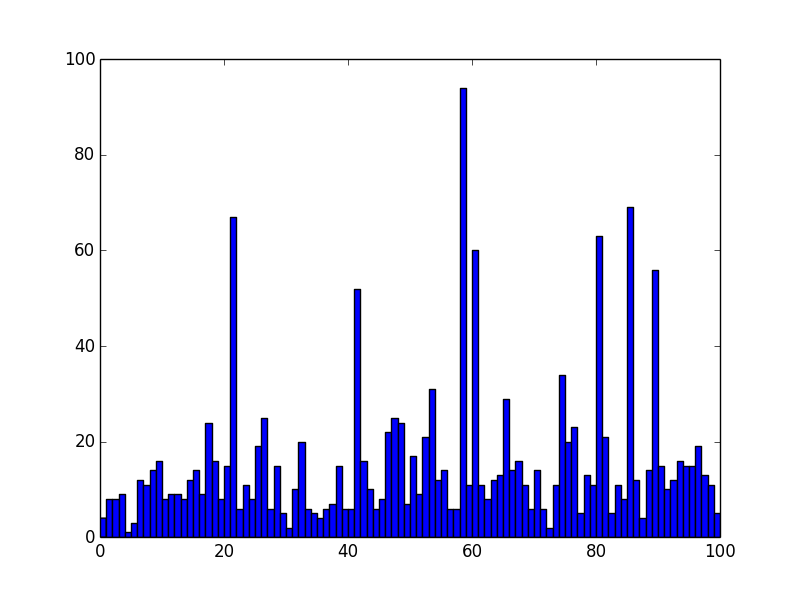
\includegraphics[scale=0.18]{132_sig.png}
    \caption{Signature}
    \label{fig:Sig}
      \end{center}
    \end{minipage}
    \hfill
    \begin{minipage}[c]{.55\linewidth}
      \begin{center}
        \begin{itemize}
            \item Signature
            \begin{itemize}
                \item Design histogram in function of assignment of the vectors.
            \end{itemize}
        \end{itemize}
      \end{center}
    \end{minipage}
\end{figure}


\end{frame}
%%-----------------------------------------------------------------------------------------

\begin{frame} \frametitle{CLEF}

\end{frame}
%%-----------------------------------------------------------------------------------------

\begin{frame} \frametitle{Process flow}

\begin{itemize}
    \item Main function which control all the process
    \begin{itemize}
        \item Create the tree structure.
        \item Allows the choice of descriptors.
    \end{itemize}
\end{itemize}

\begin{figure}[ht]
        \centering
        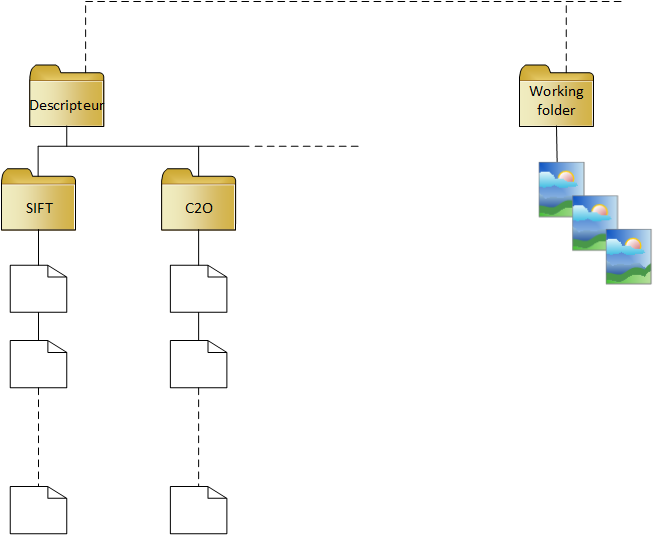
\includegraphics[scale=0.25]{arborescence.png}
        \caption{Tree structure}
        \label{fig:img_arbo}
    \end{figure}


\end{frame}
%%-----------------------------------------------------------------------------------------

\section{Results and Discussion}
\begin{frame} \frametitle{Results}
%%-----------------------------------------------------------------------------------------
\begin{itemize}
    \item Reduce data-base of 100 images composed of only 4 species.
    \item Compare the two descriptors SIFT and C$_2$O.
\end{itemize}

\begin{figure}[htbp]
    \resizebox{3.5cm}{!}{
    \begin{minipage}[c]{.55\linewidth}
      \begin{center}
        \begin{table}[H]
        \centering
        \caption{SIFT result}
        \label{tab1}
        \begin{tabular}{|l|l|l|l|l|}
        \hline
        ID & Training Base & Test Base & Correct & Accuracy \\ \hline
        173 & 17 & 8 & 4 & 50\% \\ \hline
        1102 & 22 & 3 & 1 & 33\% \\ \hline
        1889 & 16 & 9 & 1 & 11\% \\ \hline
        2717 & 15 & 10 & 7 & 70\% \\ \hline
        Total & 70 & 30 & 9 & / \\ \hline
        \end{tabular}
        \end{table}
      \end{center}
    \end{minipage}}

    \resizebox{3.5cm}{!}{
    \begin{minipage}[c]{.55\linewidth}
      \begin{center}
            \begin{table}[H]
            \caption{C$_2$O result}
            \label{tab2}
            \begin{tabular}{|l|l|l|l|l|}
            \hline
            ID & Training Base & Test Base & Correct & Accuracy \\ \hline
            173 & 17 & 8 & 1 & 12.5\% \\ \hline
            1102 & 22 & 3 & 1 & 33\% \\ \hline
            1889 & 16 & 9 & 0 & 0\% \\ \hline
            2717 & 15 & 10 & 7 & 70\% \\ \hline
            Total & 70 & 30 & 9 & / \\ \hline
            \end{tabular}
            \end{table}
      \end{center}
    \end{minipage}}
\end{figure}

\end{frame}
%%-----------------------------------------------------------------------------------------

\begin{frame} \frametitle{Discussion}

\begin{itemize}
    \item Classification
    \vspace{0.3cm}
    \begin{itemize}
        \item To much reducing on the K-means (100 words).
        \vspace{0.15cm}
        \item Euclidean distance not the most efficient or adapt.
    \end{itemize}
    \vspace{0.7cm}
    \item C$_2$O
    \vspace{0.3cm}
    \begin{itemize}
        \item The concatenation way is not optimal.
    \end{itemize}
\end{itemize}
\end{frame}
%%-----------------------------------------------------------------------------------------

\section{Project Management}
\begin{frame} \frametitle{SCRUM method}
%%-----------------------------------------------------------------------------------------

\end{frame}
%%-----------------------------------------------------------------------------------------

\section{Conclusion}
\begin{frame} \frametitle{Conclusion}
%%-----------------------------------------------------------------------------------------

\end{frame}
%%-----------------------------------------------------------------------------------------


\section{}
\begin{frame} \frametitle{}
%%-----------------------------------------------------------------------------------------
    \begin{center}
        Thanks for attention
    \end{center}
\end{frame}
%%-----------------------------------------------------------------------------------------


\end{document}

